\documentclass[journal,12pt,twocolumn]{IEEEtran}
%
\usepackage{setspace}
\usepackage{gensymb}
\singlespacing
\usepackage[cmex10]{amsmath}
\usepackage{siunitx}
\usepackage{amsthm}
\usepackage{float}
\usepackage{mathrsfs}

\usepackage{txfonts}
\usepackage{stfloats}

\usepackage{steinmetz}
\usepackage{cite}
\usepackage{cases}
\usepackage{subfig}
\usepackage{longtable}
\usepackage{multirow}
\usepackage{enumitem}
\usepackage{mathtools}
\usepackage{tikz}
\usepackage{circuitikz}
\usepackage{verbatim}
\usepackage{tfrupee}
\usepackage[breaklinks=true]{hyperref}
\usepackage{tkz-euclide} % loads  TikZ and tkz-base
\usetikzlibrary{calc,math}
\usetikzlibrary{fadings}
\usepackage{listings}
    \usepackage{color}                                            %%
    \usepackage{array}                                            %%
    \usepackage{longtable}                                        %%
    \usepackage{calc}                                             %%
    \usepackage{multirow}                                         %%
    \usepackage{hhline}                                           %%
    \usepackage{ifthen}                                           %%
  %optionally (for landscape tables embedded in another document): %%
    \usepackage{lscape}     
\usepackage{multicol}
\usepackage{chngcntr}
\DeclareMathOperator*{\Res}{Res}

\renewcommand\thesection{\arabic{section}}
\renewcommand\thesubsection{\thesection.\arabic{subsection}}
\renewcommand\thesubsubsection{\thesubsection.\arabic{subsubsection}}

\renewcommand\thesectiondis{\arabic{section}}
\renewcommand\thesubsectiondis{\thesectiondis.\arabic{subsection}}
\renewcommand\thesubsubsectiondis{\thesubsectiondis.\arabic{subsubsection}}

\hyphenation{op-tical net-works semi-conduc-tor}
\def\inputGnumericTable{}                                 %%

\lstset{
%language=C,
frame=single, 
breaklines=true,
columns=fullflexible
}
\begin{document}
%


\newtheorem{theorem}{Theorem}[section]
\newtheorem{problem}{Problem}
\newtheorem{proposition}{Proposition}[section]
\newtheorem{lemma}{Lemma}[section]
\newtheorem{corollary}[theorem]{Corollary}
\newtheorem{example}{Example}[section]
\newtheorem{definition}[problem]{Definition}
\newcommand{\BEQA}{\begin{eqnarray}}
\newcommand{\EEQA}{\end{eqnarray}}
\newcommand{\define}{\stackrel{\triangle}{=}}
\bibliographystyle{IEEEtran}
\providecommand{\mbf}{\mathbf}
\providecommand{\pr}[1]{\ensuremath{\Pr\left(#1\right)}}
\providecommand{\qfunc}[1]{\ensuremath{Q\left(#1\right)}}
\providecommand{\sbrak}[1]{\ensuremath{{}\left[#1\right]}}
\providecommand{\lsbrak}[1]{\ensuremath{{}\left[#1\right.}}
\providecommand{\rsbrak}[1]{\ensuremath{{}\left.#1\right]}}
\providecommand{\brak}[1]{\ensuremath{\left(#1\right)}}
\providecommand{\lbrak}[1]{\ensuremath{\left(#1\right.}}
\providecommand{\rbrak}[1]{\ensuremath{\left.#1\right)}}
\providecommand{\cbrak}[1]{\ensuremath{\left\{#1\right\}}}
\providecommand{\lcbrak}[1]{\ensuremath{\left\{#1\right.}}
\providecommand{\rcbrak}[1]{\ensuremath{\left.#1\right\}}}
\theoremstyle{remark}
\newtheorem{rem}{Remark}
\newcommand{\sgn}{\mathop{\mathrm{sgn}}}
\providecommand{\abs}[1]{\left\vert#1\right\vert}
\providecommand{\abs}[1]{\lvert#1\rvert} 
\providecommand{\res}[1]{\Res\displaylimits_{#1}} 
\providecommand{\norm}[1]{\left\lVert#1\right\rVert}
%\providecommand{\norm}[1]{\lVert#1\rVert}
\providecommand{\mtx}[1]{\mathbf{#1}}
\providecommand{\mean}[1]{E\left[ #1 \right]}
\providecommand{\fourier}{\overset{\mathcal{F}}{ \rightleftharpoons}}
%\providecommand{\hilbert}{\overset{\mathcal{H}}{ \rightleftharpoons}}
\providecommand{\system}{\overset{\mathcal{H}}{ \longleftrightarrow}}
	%\newcommand{\solution}[2]{\textbf{Solution:}{#1}}
\newcommand{\solution}{\noindent \textbf{Solution: }}
\newcommand{\cosec}{\,\text{cosec}\,}
\providecommand{\dec}[2]{\ensuremath{\overset{#1}{\underset{#2}{\gtrless}}}}
\newcommand{\myvec}[1]{\ensuremath{\begin{pmatrix}#1\end{pmatrix}}}
\newcommand{\mydet}[1]{\ensuremath{\begin{vmatrix}#1\end{vmatrix}}}
\numberwithin{equation}{subsection}
\makeatletter
\@addtoreset{figure}{problem}
\makeatother
\let\StandardTheFigure\thefigure
\let\vec\mathbf
\renewcommand{\thefigure}{\theproblem}
\def\putbox#1#2#3{\makebox[0in][l]{\makebox[#1][l]{}\raisebox{\baselineskip}[0in][0in]{\raisebox{#2}[0in][0in]{#3}}}}
     \def\rightbox#1{\makebox[0in][r]{#1}}
     \def\centbox#1{\makebox[0in]{#1}}
     \def\topbox#1{\raisebox{-\baselineskip}[0in][0in]{#1}}
     \def\midbox#1{\raisebox{-0.5\baselineskip}[0in][0in]{#1}}
\vspace{3cm}
\title{ASSIGNMENT-8}
\author{A.TEJASRI}
\maketitle
\newpage
\bigskip
\renewcommand{\thefigure}{\theenumi}
\renewcommand{\thetable}{\theenumi}
%
Download all python codes from 
\begin{lstlisting}
https://github.com/tejasri3657/Assignment-8/blob/main/Assignment-8(a).py
\end{lstlisting}
%
Latex-tikz codes from 
%
\begin{lstlisting}
https://github.com/tejasri3657/Assignment-8/blob/main/main.tex
\end{lstlisting}
%
\section{QUESTION No-2.26(Vectors)}
Find the coordinates of a point which divides the line segment joining the points \myvec{1 \\ -2 \\ 3} and \myvec{3 \\ 4 \\ -5} in the ratio $2:3$.
\begin{enumerate}
\item Internally and 
\item Externally
\end{enumerate}
\section{Solution}
Given 
\begin{align}
  \vec{A} = \myvec{1 \\ -2 \\ 3}, \vec{B}=\myvec{3 \\ 4\\ -5} \label{eq:1}
\end{align}
(1). The coordinates of point $\vec{P}$ dividing the line $AB$ in the ratio $m:n$ is given by 
\begin{align}
\vec{P} = \frac{m\vec{B}+n\vec{A}}{m+n}  \label{2.0.2}
\end{align}
Given that the point $\vec{P}$ divides $AB$ in the ratio $2:3$, now to find $\vec{P}$ we use \eqref{eq:1},
\begin{align}
\vec{P}=\frac{2\myvec{3\\4\\-5}+3\myvec{1\\-2\\3}}
{(2+3)}
\\
\implies\vec{P}=\myvec{{\frac{9}{5}} \\ {\frac{2}{5}} \\ {\frac{-1}{5}}}
\end{align}
(2). The coordinates of point $\vec{Q}$ dividing the line $AB$ in the ratio $m:n$ is given by 
\begin{align}
 \vec{Q} = \frac{m\vec{B}-n\vec{A}}{m+n}  \label{2.0.5}
\end{align}
Given that the point $\vec{Q}$ divides $AB$ in the ratio $2:3$, now to find $\vec{Q}$ we use \eqref{eq:1},
\begin{align}
\vec{Q}=\frac{2\myvec{3\\4\\-5}-3\myvec{1\\-2\\3}}
{(2-3)}
\\
\implies\vec{Q}=\myvec{-3\\-14\\19}
\end{align}

\numberwithin{figure}{section}
\begin{figure}[H]
Plot of the line Internally :
    \centering
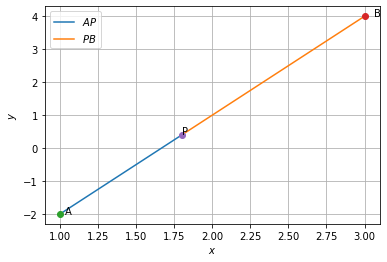
\includegraphics[width=\columnwidth]{internally.png}
    \caption{INTERNALLY}
    \label{fig:Internally.}
\end{figure} 
\numberwithin{figure}{section}
\begin{figure}[H]
Plot of the line Externally :
    \centering
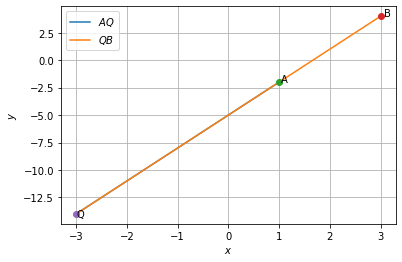
\includegraphics[width=\columnwidth]{externally.png}
    \caption{EXTERNALLY}
    \label{fig:EXTERNALLY.}
\end{figure}  
\end{document}
